The results for this experiment are as expected.
All three algorithms find the optimal value within the time limit.
The RLS performs better than the (1+1) EA because it does only single bit flips.
The $pmut_{-3.25}$ performs better than the standard (1+1) EA although flipping more bits on average.
This is most likely cause by the few steps where $pmut$ flips many bits which increase the average.
But $pmut$ most likely chooses to flip only one bit more often as the (1+1) EA.\newline
For this comparison neither of the algorithms failed to find one of the two optimal solutions.
The following table lists the amount of iterations the algorithms needed to find an optimal solution.

\begin{tabular}[h]{ccccccccc}
      input size     & 20  & 50  & 100  & 500  & 1000  & 5000   & 10000  & 50000   \\\hline
      RLS            & 56  & 187 & 446  & 3050 & 6725  & 42056  & 90485  & 537292  \\
      (1+1) EA (1/n) & 131 & 438 & 1059 & 7435 & 16963 & 106410 & 230310 & 1379632 \\
      pmut (-3.25)   & 82  & 277 & 667  & 4666 & 10432 & 66450  & 142919 & 846722  \\
      pmut (-3.5)    & 77  & 265 & 642  & 4393 & 9930  & 62337  & 137048 & 801570  \\
\end{tabular}

The RLS performs the best closely follow by both $pmut$ variants.
The standard (1+1) EA performs a bit worse than the other three algorithms and approaches $en\ln(n)$ instead of staying close to $n\ln(n)$.

\begin{figure}[h]
      \caption{Runtime for OneMax equivalent with a $n\ln(n)$ scale}
      \centering
      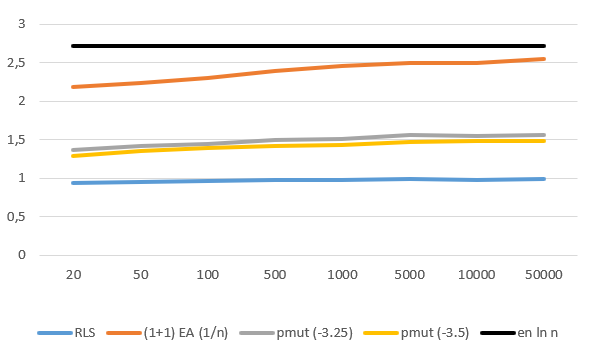
\includegraphics[width=0.7\textwidth]{figures/images/oneMaxMultipleN.png}\label{fig:onemaxNlogNBound}
\end{figure}